\documentclass[12pt,letterpaper]{article}
\usepackage[margin=.7in,headheight=18pt,headsep=17pt,footskip=28pt]{geometry}
\usepackage{tikz,fancyhdr,amssymb}
\usetikzlibrary{arrows.meta}
\pdfmapfile{+cm.map}\pdfmapfile{+cmextra.map}\pdfmapfile{+symbols.map}\pdfmapfile{+latxfont.map}
\renewcommand{\familydefault}{\sfdefault}
\setlength{\parindent}{0pt}\setlength{\parskip}{9pt}
\pagestyle{fancy}\fancyhf{}
\fancyhead[L]{\small Week 68 / How many ways out / Grades 3--5}
\fancyfoot[L]{\footnotesize Bellingham Math Circle / Week 68 / GGT68-S-v1}
\fancyfoot[R]{\footnotesize\thepage}\renewcommand{\headrulewidth}{.4pt}

\newcommand{\problem}[2]{\par\textbf{Problem #1:} #2\par}
\newcommand{\roadline}{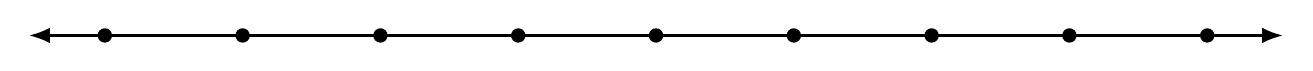
\begin{tikzpicture}[x=1.75cm,y=1cm]
\draw[{Latex}-{Latex},line width=1pt] (-4.55,0)--(4.55,0);\foreach \i in {-4,...,4}\fill (\i,0) circle (2.6pt);\end{tikzpicture}}
\newcommand{\ladder}{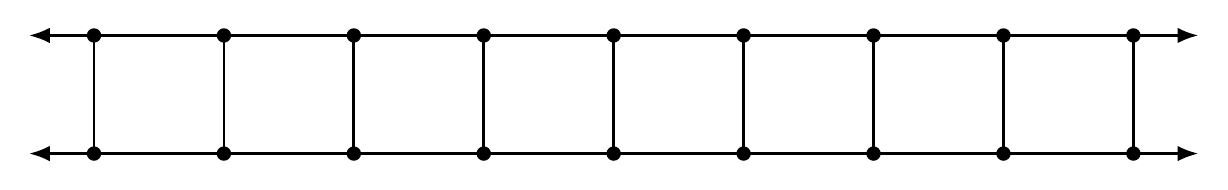
\begin{tikzpicture}[x=1.65cm,y=1.5cm]
\foreach \y in {0,1}{\draw[{Latex}-{Latex},line width=1pt] (-4.5,\y)--(4.5,\y);}
\foreach \x in {-4,...,4}{\draw[line width=1pt] (\x,0)--(\x,1);\foreach \y in {0,1}\fill (\x,\y) circle (2.6pt);}\end{tikzpicture}}
\newcommand{\grid}{\draw[gray!70,line width=.6pt,step=1] (-3,-3) grid (3,3);
\foreach \x in {-3,...,3}{\draw[-{Latex},gray!70] (\x,3)--(\x,3.5);\draw[-{Latex},gray!70] (\x,-3)--(\x,-3.5);}
\foreach \y in {-3,...,3}{\draw[-{Latex},gray!70] (-3,\y)--(-3.5,\y);\draw[-{Latex},gray!70] (3,\y)--(3.5,\y);}
\foreach \x in {-3,...,3}\foreach \y in {-3,...,3}\fill (\x,\y) circle (1.8pt);}
\begin{document}
Cover dots with counters. A covered dot and every road touching it are closed. Before lifting counters, mark their dots with X. One partner places the blockers; the other traces open routes. Swap jobs between attempts.
\begin{center}
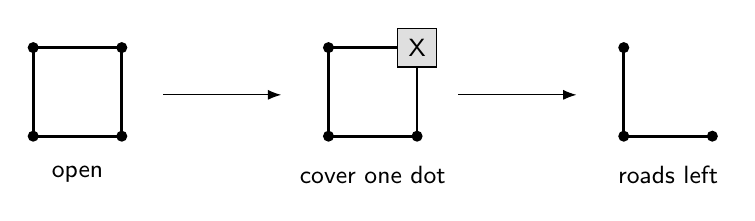
\begin{tikzpicture}[x=.75cm,y=.75cm,font=\small]
\foreach \s in {0,5,10}{\begin{scope}[shift={(\s,0)}]
\ifnum\s=10\draw[line width=1pt] (0,1.5)--(0,0)--(1.5,0);\else\draw[line width=1pt] (0,0) rectangle (1.5,1.5);\fi
\foreach \p in {(0,0),(0,1.5),(1.5,0)}\fill \p circle (2pt);
\ifnum\s<10\fill (1.5,1.5) circle (2pt);\fi
\ifnum\s=5\node[draw,fill=gray!25,minimum size=14pt] at (1.5,1.5){X};\fi
\end{scope}}
\node at (.75,-.65){open};\node at (5.75,-.65){cover one dot};\node at (10.75,-.65){roads left};
\draw[-{Latex}] (2.2,.7)--(4.2,.7);\draw[-{Latex}] (7.2,.7)--(9.2,.7);
\end{tikzpicture}
\end{center}
On the maps below, arrows mean the road pattern keeps going forever. A piece counts as a \textbf{forever piece} only if it keeps going beyond every distance. A trapped finite piece does not count.
\problem{1}{On each line, use the stated number of blockers. Make as many forever pieces as you can. Circle any trapped pieces.}
\vspace{.2in}
\roadline\par 1 blocker\hfill Forever pieces: \rule{.7in}{.4pt}\par
\vspace{.45in}
\roadline\par 2 blockers\hfill Forever pieces: \rule{.7in}{.4pt}\par
\vspace{.45in}
\roadline\par 4 blockers\hfill Forever pieces: \rule{.7in}{.4pt}\par
\vspace{.15in}
\problem{2}{Place four blockers on a fresh line so that exactly two pieces are trapped.}
\vspace{.2in}\roadline
\newpage
The ladder has two endless rails. A rung joins them at every dot pair, including beyond the arrows.
\problem{3}{One partner covers one dot and chooses two open dots. The other tries to join them by an open route. Swap jobs, then allow two blocked dots. Keep one attempt that separates forever pieces and one that leaves them together.}
\vspace{.3in}
\begin{center}\ladder\end{center}
\vspace{.5in}
\begin{center}\ladder\end{center}
\vspace{.3in}
\problem{4}{Can four blocked dots make three separate forever pieces on the ladder? Show a placement that works, or explain why no placement can.}
\vspace{.25in}
\begin{center}\ladder\end{center}
\vspace{.35in}\rule{\linewidth}{.4pt}\par\vspace{.4in}\rule{\linewidth}{.4pt}
\newpage
The square grid continues in every direction, with the same rows, columns, and connecting roads. Routes may leave the printed window.
\problem{5}{On the left grid, use four blockers to trap an open dot. On the right grid, the five X dots are closed. Join P to Q by an open route. Which pieces on each map keep going forever?}
\vspace{.2in}
\begin{center}
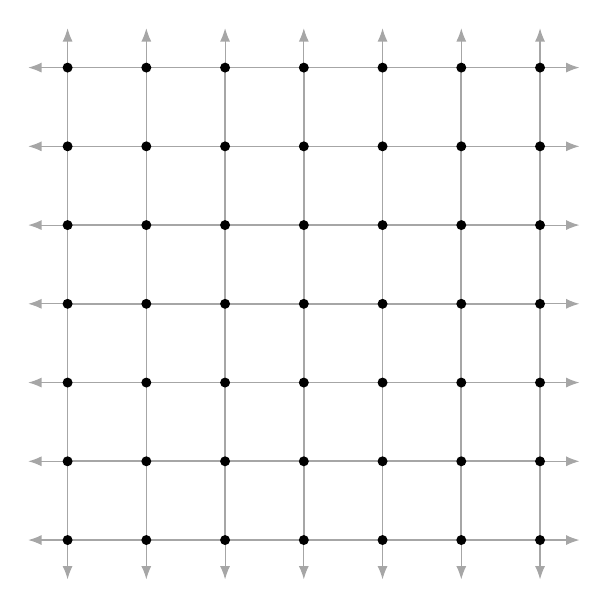
\begin{tikzpicture}[x=1cm,y=1cm]\grid\end{tikzpicture}\hfill
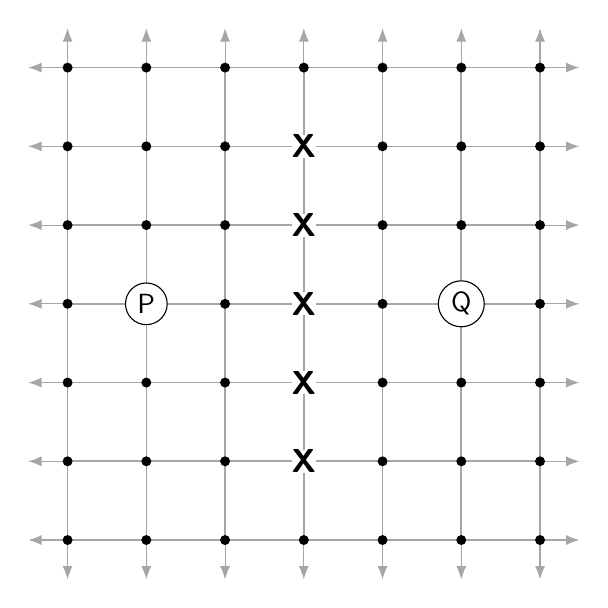
\begin{tikzpicture}[x=1cm,y=1cm]\grid
\foreach \y in {-2,...,2}\node[fill=white,inner sep=0pt,font=\bfseries\large] at (0,\y){X};
\node[draw,circle,fill=white,inner sep=2pt] at (-2,0){P};\node[draw,circle,fill=white,inner sep=2pt] at (2,0){Q};
\end{tikzpicture}
\end{center}
\vspace{.2in}
\problem{6}{Can any finite collection of blocked dots split the endless grid into two forever pieces? Draw or explain your answer. Your answer must still work beyond the edge of the page.}
\vspace{.35in}\rule{\linewidth}{.4pt}\par\vspace{.45in}\rule{\linewidth}{.4pt}\par\vspace{.45in}\rule{\linewidth}{.4pt}\par\vspace{.45in}\rule{\linewidth}{.4pt}
\newpage
On this branching map, every tip keeps splitting into two new branches forever. Branches never join again. Each line between dots is one road.
\problem{7}{Cover the center dot. Next cover all dots one road from the center too. Next cover all dots two roads from the center too. Count the separate forever pieces each time.}
\begin{center}
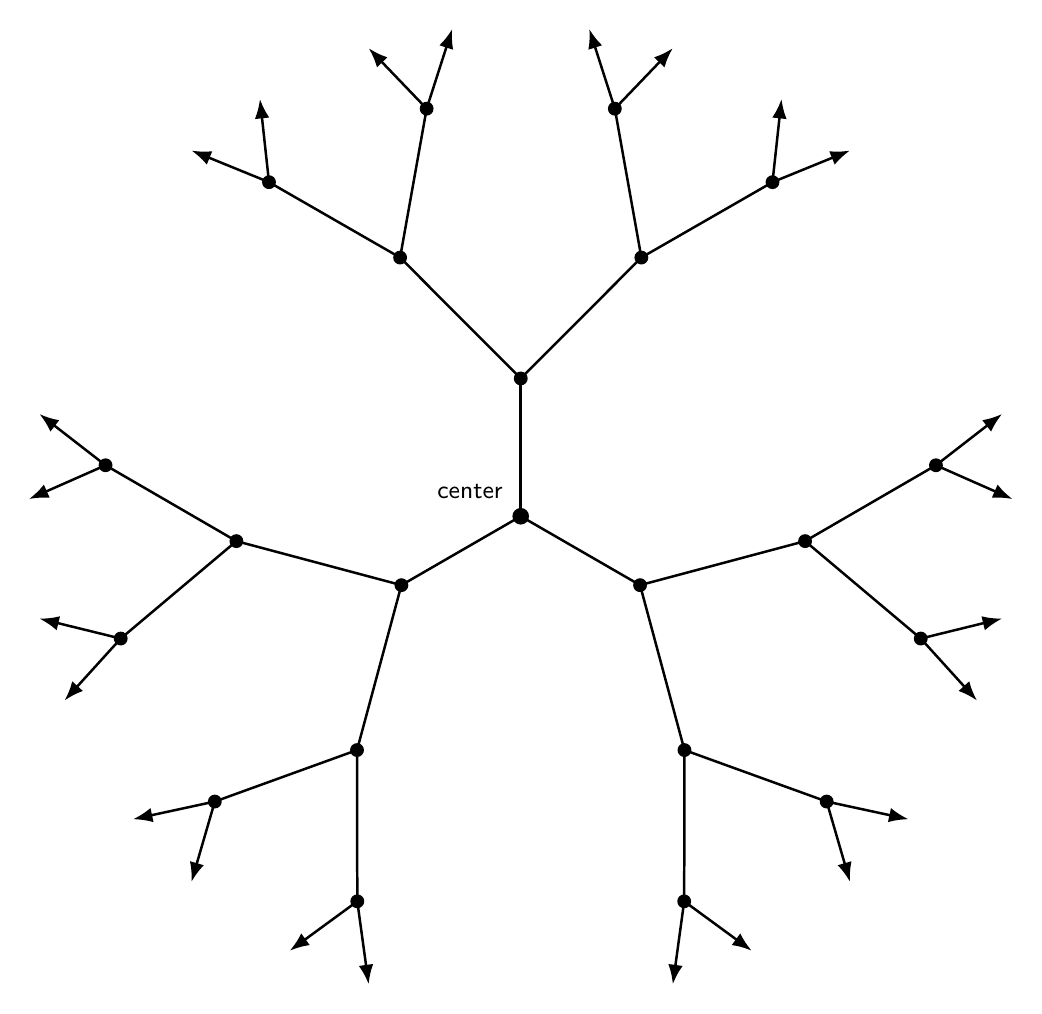
\begin{tikzpicture}[x=1.25cm,y=1.25cm]
\coordinate (o) at (0,0);\node[above left=3pt,font=\small] at (o){center};
\foreach \a in {90,210,330}{
\coordinate (a\a) at (\a:1.4);\draw[line width=.9pt] (o)--(a\a);\fill (a\a) circle (2.5pt);
\foreach \b in {-25,25}{\pgfmathsetmacro{\ab}{\a+\b}
\coordinate (b\a\b) at (\ab:2.9);\draw[line width=.9pt] (a\a)--(b\a\b);\fill (b\a\b) circle (2.5pt);
\foreach \c in {-12,12}{\pgfmathsetmacro{\abc}{\ab+\c}
\coordinate (c\a\b\c) at (\abc:4.25);\draw[line width=.9pt] (b\a\b)--(c\a\b\c);\fill (c\a\b\c) circle (2.5pt);
\foreach \d in {-5,5}{\pgfmathsetmacro{\abcd}{\abc+\d}\draw[-{Latex},line width=.9pt] (c\a\b\c)--(\abcd:5.0);}
}}}\fill (o) circle (3pt);
\end{tikzpicture}
\end{center}
Center only: \rule{.6in}{.4pt}\hfill Through 1 road: \rule{.6in}{.4pt}\hfill Through 2 roads: \rule{.6in}{.4pt}
\problem{8}{How many forever pieces would remain after blocking through 3 roads? Explain how the count changes as the blocked distance keeps growing.}
\vspace{.25in}\rule{\linewidth}{.4pt}\par\vspace{.3in}\rule{\linewidth}{.4pt}
\end{document}
